\documentclass[12pt]{article}
\usepackage[utf8]{inputenc}
\usepackage[a4paper, left=3cm, right=2cm, top=3cm, bottom=2cm]{geometry}

\usepackage{indentfirst}
\usepackage{amsmath}
\usepackage[T1]{fontenc}
\usepackage{listings}
\usepackage{minted}

% adicionar suporte ao idioma pt-br
\usepackage[brazil]{babel}

% Utilização de imagens
\usepackage{graphicx} 
\usepackage{wrapfig}

% Possibilita o uso do H no posicionamento de figuras
\usepackage{float} 

% das referências
\usepackage[square,sort,comma,numbers]{natbib}
\usepackage{url}
\usepackage{hyperref}

% permite criação região de comentário
\usepackage{comment}
\usepackage[brazil]{babel} % \usepackage[latin1]{inputenc}
\usepackage{a4wide}
\setlength{\oddsidemargin}{-0.2in}
% % \setlength{\oddsidemargin}{0.2in}
\setlength{\evensidemargin}{-0.2in}
% % \setlength{\evensidemargin}{0.5in}
% % \setlength{\textwidth}{5.5in}
\setlength{\textwidth}{6.5in}
\setlength{\topmargin}{-1.2in}
\setlength{\textheight}{10in}
\usepackage[]{amsfonts} \usepackage[]{amsmath}
\usepackage[]{amssymb} \usepackage[]{latexsym}
\usepackage{graphicx,color} \usepackage{amsthm}
\usepackage{mathrsfs} \usepackage{url}
\usepackage{cancel} \usepackage[inline]{enumitem}
\usepackage{xifthen} \usepackage{tikz}
\usetikzlibrary{automata,arrows,positioning,calc}

\numberwithin{equation}{section}

\setlength{\parindent}{12 pt}

\title{Modelos Matemáticos Predador-Presa no Controle de Pragas em Plantações de Citros e Cana-de-açúcar}
\author{Ezequiel de Braga Santos, Pedro Lima Garcia \\ Escola de Matemática Aplicada, FGV - EMAp \\ Rio de Janeiro/RJ.}

\date{}

\begin{document}

\setcounter{page}{1}
\pagenumbering{arabic}

% Estrutura do trabalho

\maketitle

\section{Introdução}

O Brasil é o maior produtor de frutas cítricas e cana-de-açúcar do mundo, sendo responsável por produzir cerca de 20 milhões de toneladas de citros e mais de 600 milhões de toneladas de cana-de-açúcar nos últimos anos. No entanto, essas plantações são atacadas por algumas pragas, gerando sérios prejuízos à produção. As primeiras são atingidas pela morte súbita dos citros (PEIXOTO,
BARROS, BASSANEZI, 2005) \cite{mp_lb_rb_2005}, doença que chegou ao extremo de provocar a morte de grandes plantações no estado de São Paulo. Já a cana-de-açúcar é afetada pela \textit{Diatraea saccharalis} (JESUS, LIMA, 2017) \cite{ij_al_2017}, que gera inúmeras falhas na germinação, morte das gemas e perda de peso, diminuindo a pureza.

No caso da cana-de-açúcar, a \textit{Diatraea saccharalis}, conhecida como broca da cana-de-açúcar, passa a maior parte do tempo dentro da cana, dificultando a ação de agentes químicos. Como consequência, o controle biológico tem sido a forma mais eficiente de combate, com a utilização de outros insetos predadores presentes no canavial. Já nos citros, pesquisadores acreditam que a doença é causada por um vírus transmitido por insetos conhecidos como pulgões, os quais possuem as joaninhas como predadores naturais mais conhecidos.

Nesse sentido, a Modelagem Matemática é uma ferramenta importante para encontrar maneiras de controlar ou resolver tais problemas. Os modelos matemáticos para esse fim tiveram origem com Lotka em 1925 e Volterra em 1926, que propuseram um modelo que foi, posteriormente, denominado modelo de Lotka-Volterra, utilizado para descrever a dinâmica de sistemas do tipo predador-presa, onde uma das espécies é predadora da outra, a presa, que se alimenta de outro tipo de alimento. Esse modelo já foi utilizado para modelagem do controle biológico do controle de pragas em algumas plantações, como podemos ver no artigo de Viviane Noronha e Rosana Ferreira \cite{vn_rf_2021}, que trata do controle biológico de maneira mais geral na frutífera brasileira, e também no artigo de I. Jesus  A. D. Lima \cite{ij_al_2017}, o qual faz uma abordagem aplicada à cana-de-açúcar.

Além disso, podemos citar o modelo de Holling-Tanner que, diferentemente do modelo anterior, ``leva em consideração o efeito predação e as capacidades de suportes das populações de presas e predadores'' (SILVEIRA, GARCIA, 2020) \cite{gs_rg_2020}, proposto no artigo de Magda S. Peixoto, Laécio C. Barros e Rodney C. Bassanezi para o controle de praga nos citros \cite{mp_lb_rb_2005}. 

Em nosso trabalho, além dos modelos supracitados, vamos propor uma análise com o modelo de Rosenzweig-MacArthur, que considera fatores adicionais na população de predadores como, por exemplo, uma taxa de mortalidade \cite{id_mg_r_2021}, devido outros agentes. Em nossa modelagem, iremos admitir a existência de um superpredador sem capacidade de reprodução, o qual provoca uma taxa de mortalidade nos predadores. A seguir, vamos apresentar os modelos citados para descrever a dinâmica predador-presa, bem como utilizá-los para modelar os problemas relatados.

\newpage

\section{Metodologia}

\subsection{Modelo de Lotka-Volterra}

Em sua dissertação de mestrado, Isaías de Jesus (2018) \cite{ij_2018} utilizou o modelo de Lotka-Volterra para modelar o controle biológico de pragas da cana-de-açúcar. A praga em questão era \textit{Diatraea Saccharalis} (broca da cana-de-açúcar) e seu predador era \textit{Cotesia flavipes} (vespa). Através dessa modelagem ele pôde encontrar computacionalmente a situação de equilíbrio em diferentes cenários e definir a estratégia de controle mais adequada. Eis abaixo as equações do modelo e seus parâmetros:

$$\left\{
\begin{array}{l}
\dfrac{dx}{dt}=x(a-by)\\
\dfrac{dy}{dt}=y(cx-d)
\end{array}
\right.$$

\begin{itemize}
    \item $x=x(t)$: população de brocas (em função do tempo); 
    \item $y=y(t)$: população de vespas (em função do tempo);
    \item $a$: taxa de crescimento da população de brocas na ausência de vespas;
    \item $b$: taxa de decrescimento da população de brocas devido aos encontros com vespas;
    \item $c$: taxa de crescimento da população de vespas devido à predação;
    \item $d$: taxa de decrescimento da população de vespas na ausência de brocas.
\end{itemize}

\

\subsubsection{Análise dimensional}

Vamos atribuir grandezas $M$ para massa e $T$ para tempo.

As grandezas de $x$ e $y$ serão massas, pois representam as populações. Por ser uma taxa, $a$ terá grandeza $\frac{1}{T}$. Para que $-by$ possa ser somado a $a$, $b$ deverá ter grandeza $\frac{1}{MT}$. Disso conclui-se que $\frac{dx}{dt}$ tem grandeza $\frac{M}{T}$.

Em $\frac{dy}{dt}$ ocorre algo bem semelhante. As grandezas de $x$ e $y$ continuam sendo massas. Por ser uma taxa, $d$ terá grandeza $\frac{1}{T}$. Logo, para que $cx$ possa ser somado a $-d$, $c$ deverá ter grandeza $\frac{1}{MT}$. Disso resulta que $\frac{dx}{dt}$ tem grandeza $\frac{M}{T}$.

Faz sentido que as grandezas obtidas para $\frac{dx}{dt}$ e $\frac{dy}{dt}$ sejam essas, já que as populações variam ao longo do tempo.

\begin{center}
\begin{tabular}{| c | c | c |}
\hline
%& \multicolumn{3}{c|}{Notas}\\
%\cline{2 - 7} % linha horizontal entre as colunas
% 2 e 4
Parâmetro & Unidade & Descrição\\
\hline
$x=x(t)$ & $M$ & População de presas\\
$y=y(t)$ & $M$ & População de predadores\\
$a$ & $1/T$ & Taxa de crescimento de presas na ausência de predadores\\
$b$ & $1/MT$ & Taxa de decrescimento de presas devido à predação\\
$c$ & $1/MT$ & Taxa de crescimento de predadores devido à predação\\
$d$ & $1/T$ & Taxa de decrescimento de predadores na ausência de presas\\
\hline
\end{tabular}
\end{center}

\newpage

\subsection{Modelo de Holling-Tanner}

Para estudar a interação entre pulgões (\textit{Toxoptera citricida}) e joaninhas (\textit{Cycloneda sanguinea}), Magda Peixoto, Laécio Barros e Rodney Bassanezi (2005) \cite{mp_lb_rb_2005} ajustaram em seu artigo o modelo predador-presa de Holling-Tanner para interpretar biologicamente seus parâmetros. Desse modo, o controle da praga pulgão na plantação de citros pôde ser feito por meio de sua predadora, a joaninha.

$$\left\{
\begin{array}{l}
\dfrac{dx}{dt}=rx\left(1-\dfrac{x}{K}\right)-\dfrac{mxy}{A+x}\\
\dfrac{dy}{dt}=sy\left(1-\dfrac{cy}{x}\right)
\end{array}
\right.$$

\begin{itemize}
    \item $x=x(t)$: população de pulgões (em função do tempo); 
    \item $y=y(t)$: população de joaninhas (em função do tempo);
    \item $r$: taxa de crescimento intrínseco dos pulgões;
    \item $K$: capacidade suporte dos pulgões na ausência de joaninhas;
    \item $m$: número máximo de pulgões que podem ser consumidos por uma joaninha em cada unidade de tempo;
    \item $A$: número de pulgões necessários para atingir metade do número máximo $m$;
    \item $s$: taxa de crescimento intrínseco das joaninhas;
    \item $c$: medida da qualidade alimentícia proporcionada pelo pulgão para sua conversão em nascimento de joaninhas.
\end{itemize}

\subsubsection{Análise dimensional}

Vamos atribuir grandezas $M$ para massa e $T$ para tempo.

As grandezas de $x$ e $y$ serão massas, pois representam as populações. Por ser uma taxa, $r$ terá grandeza $\frac{1}{T}$. Para que $\frac{x}{K}$ possa ser somado à constante 1, $K$ deverá ter grandeza $M$ (o que torna $\frac{x}{K}$ constante). $A$ deverá ter grandeza $M$ para poder ser somado a $x$. Há no numerador da segunda fração a grandeza $M^2$ de $xy$. Para que essa fração seja somada à primeira, sua grandeza deve ser também $\frac{M}{T}$, o que implica que a grandeza de $m$ deve ser $\frac{1}{T}$. Com isso conclui-se que $\frac{dx}{dt}$ tem grandeza $\frac{M}{T}$.

Em $\frac{dy}{dt}$, por ser uma taxa, $s$ terá grandeza $\frac{1}{T}$. As grandezas de $x$ e $y$ continuam sendo massas. Logo, para que a soma da fração com a constante 1 possa ocorrer, $c$ deverá ser uma constante qualquer (sem grandeza). Logo, $\frac{dy}{dt}$ tem grandeza $\frac{M}{T}$ também.

Faz sentido que as grandezas obtidas para $\frac{dx}{dt}$ e $\frac{dy}{dt}$ sejam essas, já que as populações variam ao longo do tempo.

\begin{center}
\begin{tabular}{| c | c | c |}
\hline
%& \multicolumn{3}{c|}{Notas}\\
%\cline{2 - 7} % linha horizontal entre as colunas
% 2 e 4
Parâmetro & Unidade & Descrição\\
\hline
$x=x(t)$ & $M$ & População de presas\\
$y=y(t)$ & $M$ & População de predadores\\
$r$ & $1/T$ & Taxa de crescimento intrínseco de presas\\
$K$ & $M$ & Capacidade suporte das presas na ausência dos predadores\\
$m$ & $1/T$ & Máximo de presas que podem ser consumidas por um predador\\
$A$ & $M$ & Presas necessárias para atingir $m/2$\\
$s$ & $1/T$ & Taxa de crescimento intrínseco de predadores\\
$c$ & constante & Medida da qualidade alimentícia proporcionada pela presa\\
\hline
\end{tabular}
\end{center}

\newpage

\subsection{Modelo de Rosenzweig-MacArthur}

O modelo com o qual pretendemos modelar os dois problemas anteriores é o de Rosenzweig-MacArthur, que já foi utilizado por Luiz Rodrigues, Simone Ossani e Diomar Mistro (2013) \cite{lr_so_dm_2013} para simular um sistema predador-presa em que o predador é infectado por uma doença, o que adiciona à equação uma taxa de mortalidade. 

Em nosso estudo, a simulação será feita com a inclusão de um superpredador sem capacidade de reprodução. Em cada um dos casos ele será de uma espécie predadora de vespas e joaninhas, respectivamente. A ideia é que, embora não se reproduza, sua presença no sistema cause uma redução (ainda que possivelmente temporária) de predadores. Eis abaixo as equações do sistema (os parâmetros descritos na análise dimensional serão detalhados posteriormente):

$$\left\{
\begin{array}{l}
\dfrac{dx}{dt}=rx\left(1-\dfrac{x}{K}\right)-\dfrac{mxy}{A+x}\\
\dfrac{dy}{dt}=\dfrac{cmxy}{A+x}-sy
\end{array}
\right.$$

% \begin{itemize}
%     \item $x=x(t)$: população de presas (em função do tempo); 
%     \item $y=y(t)$: população de predadores (em função do tempo);
%     \item $r$: taxa de crescimento intrínseco das presas;
%     \item $K$: capacidade suporte das presas na ausência dos predadores;
%     \item $m$: número máximo de presas que podem ser consumidas por um predador em cada unidade de tempo;
%     \item $A$: número de presas necessárias para atingir metade do número máximo $m$;
%     \item $s$: taxa de mortalidade da população de predadores;
%     \item $c$: medida da qualidade alimentícia proporcionada pela presa para sua conversão em nascimento de predadores.
% \end{itemize}

\subsubsection{Análise dimensional}

Vamos atribuir grandezas $M$ para massa e $T$ para tempo.

As grandezas de $x$ e $y$ serão massas, pois representam as populações. Por ser uma taxa, $r$ terá grandeza $\frac{1}{T}$. Para que $\frac{x}{K}$ possa ser somado à constante 1, $K$ deverá ter grandeza $M$ (o que torna $\frac{x}{K}$ constante). $A$ deverá ter grandeza $M$ para poder ser somado a $x$. Há no numerador da segunda fração a grandeza $M^2$ de $xy$. Para que essa fração seja somada à primeira, sua grandeza deve ser também $\frac{M}{T}$, o que implica que a grandeza de $m$ deve ser $\frac{1}{T}$. Com isso conclui-se que $\frac{dx}{dt}$ tem grandeza $\frac{M}{T}$.

Em $\frac{dy}{dt}$, por ser uma taxa, $s$ terá grandeza $\frac{1}{T}$. As grandezas de $x$ e $y$ continuam sendo massas. $A$ deverá ter grandeza $M$ para poder ser somado a $x$. Há no numerador da fração a grandeza $M^2$ de $xy$. Logo, $\frac{dy}{dt}$ tem grandeza $\frac{M}{T}$ também. Sabe-se que a grandeza de $m$ é $\frac{1}{T}$, então $c$ deverá ser uma constante qualquer, sem grandeza, para que a soma com $-sy$ possa ocorrer. Portato, $\frac{dy}{dt}$ tem grandeza $\frac{M}{T}$ também.

Faz sentido que as grandezas obtidas para $\frac{dx}{dt}$ e $\frac{dy}{dt}$ sejam essas, já que as populações variam ao longo do tempo.

\begin{center}
\begin{tabular}{| c | c | c |}
\hline
%& \multicolumn{3}{c|}{Notas}\\
%\cline{2 - 7} % linha horizontal entre as colunas
% 2 e 4
Parâmetro & Unidade & Descrição\\
\hline
$x=x(t)$ & $M$ & População de presas\\
$y=y(t)$ & $M$ & População de predadores\\
$r$ & $1/T$ & Taxa de crescimento intrínseco de presas\\
$K$ & $M$ & Capacidade suporte das presas na ausência dos predadores\\
$m$ & $1/T$ & Máximo de presas que podem ser consumidas por um predador\\
$A$ & $M$ & Presas necessárias para atingir $m/2$\\
$s$ & $1/T$ & Taxa de mortalidade de predadores\\
$c$ & constante & Medida da qualidade alimentícia proporcionada pela presa\\
\hline
\end{tabular}
\end{center}

\newpage

% \section{Resultados}

Utilizamos o software \textit{SageMath 9.7} para realizar as análises, definindo diferentes parâmetros e condições iniciais para os modelos apresentados.

\subsection{Equilíbrios}

\begin{center}
\begin{tabular}{| c | c | c |}
\hline
%& \multicolumn{3}{c|}{Notas}\\
%\cline{2 - 7} % linha horizontal entre as colunas
% 2 e 4
Modelo & Sistema & Equilíbrios \\
\hline
Lotka-Volterra & 
$\left\{
\begin{array}{l}
\dfrac{dx}{dt}=x(a-by)\\
\dfrac{dy}{dt}=y(cx-d)
\end{array}
\right.$ & 
\begin{tabular}{c} 
$\left[ x = 0, y = 0 \right]$ \\
$\left[ x = \frac{d}{c}, y = \frac{a}{b} \right]$
\end{tabular} \\
\hline
Holling-Tanner & 
$\left\{
\begin{array}{l}
\dfrac{dx}{dt}=rx\left(1-\dfrac{x}{K}\right)-\dfrac{mxy}{A+x}\\
\dfrac{dy}{dt}=sy\left(1-\dfrac{cy}{x}\right)
\end{array}
\right.$ & 
\begin{tabular}{c} 
$\left[ x = 0, y = 0 \right]$ \\
$\left[ x = K, y = 0 \right]$ \\
$\left[ x = -A, y = 0 \right]$ \\
$\left[ x = - \frac{ \alpha + \sqrt{\beta} }{2cr}, y = -\frac{\alpha + \sqrt{\beta}}{2c^2r} \right]$ \\
$\left[ x = - \frac{ \alpha - \sqrt{\beta} }{2cr}, y = -\frac{\alpha - \sqrt{\beta}}{2c^2r} \right]$ \\
$\alpha = (A-K)cr + Km$ \\
\scriptsize{$\beta = (A+K)^2c^2r^2 + K^2m^2 + 2(AK - K^2)cmr$}
\end{tabular} \\
\hline
Rosenzweig-MacArthur & 
$\left\{
\begin{array}{l}
\dfrac{dx}{dt}=rx\left(1-\dfrac{x}{K}\right)-\dfrac{mxy}{A+x}\\
\dfrac{dy}{dt}=\dfrac{cmxy}{A+x}-sy
\end{array}
\right.$ & 
\begin{tabular}{c} 
$\left[ x = 0, y = 0 \right]$ \\
$\left[ x = K, y = 0 \right]$ \\
$\left[ x = -A, y = 0 \right]$ \\
$\left[ x = - \frac{ As }{cm - s}, y = \frac{AKc^2mr - (A^2 + AK)crs}{Kc^2m^2 - 2Kcms + Ks^2} \right]$ 
\end{tabular} \\
\hline
\end{tabular}
\end{center}

\subsection{Simulações}

%%%%%%%%%%%%%%%%%%%%%%%%%%%%%%%%%%%%%%%%%%%%%%%%%%%%%%%%%%%
%%%%%%%%%%%%%%%%%%%%%%%%%%%%%%%%%%%%%%%%%%%%%%%%%%%%%%%%%%%
%%%%%%%%%%%%%%%%%%%% Modelo L-V %%%%%%%%%%%%%%%%%%%%%%%%%%%
%%%%%%%%%%%%%%%%%%%%%%%%%%%%%%%%%%%%%%%%%%%%%%%%%%%%%%%%%%%
%%%%%%%%%%%%%%%%%%%%%%%%%%%%%%%%%%%%%%%%%%%%%%%%%%%%%%%%%%%

\subsubsection{Modelo de Lotka-Volterra}

Define-se os parâmetros $a = 0.0126, b = 0.0000101, c = 0.00012, d = 0.1534$, calculados por Isaías de Jesus, em sua dissertação de mestrado \cite{ij_2018} (2018). Nesse caso, temos os equilíbrios $P_1 = \left(0,0 \right)$ e $P_2 = \left( \frac{3835}{3}, \frac{126000}{101} \right)$, onde a matriz Jacobiana de $P_1$ tem autovalores $-\frac{767}{5000}$ e $\frac{63}{5000}$. Logo, $P_1$ é um ponto de sela. Já a Jacobiana de $P_2$ possui autovalores complexos com parte real nula e, portanto, $P_2$ é um centro. A seguir, tem-se a simulação para diferentes condições iniciais e seus respectivos planos de fase.

\begin{figure}[H]
    \centering
    \begin{subfigure}{0.4\textwidth}
        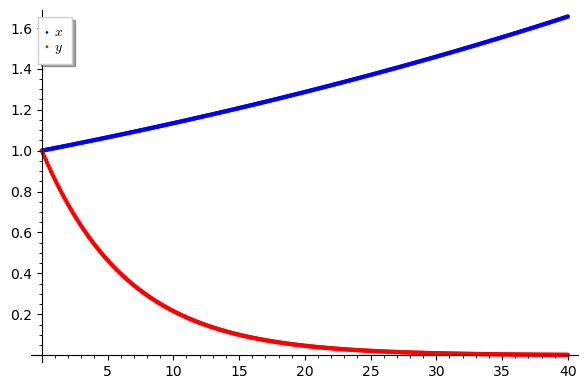
\includegraphics[scale=0.48]{figuras/LV_1.png}
        \label{fig:LV_1}
        \caption{$x_0 = y_0 = 1$}
    \end{subfigure}
    \begin{subfigure}{0.4\textwidth}
        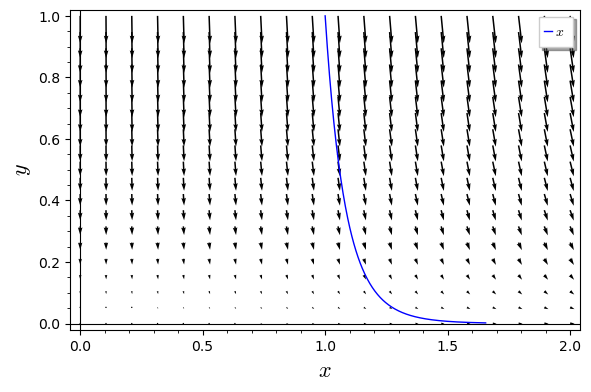
\includegraphics[scale=0.48]{figuras/LV_4.png}
        \label{fig:LV_4}
        \caption{Plano de fase}
    \end{subfigure}
\end{figure}

\begin{figure}[H]
    \centering
    \begin{subfigure}{0.4\textwidth}
        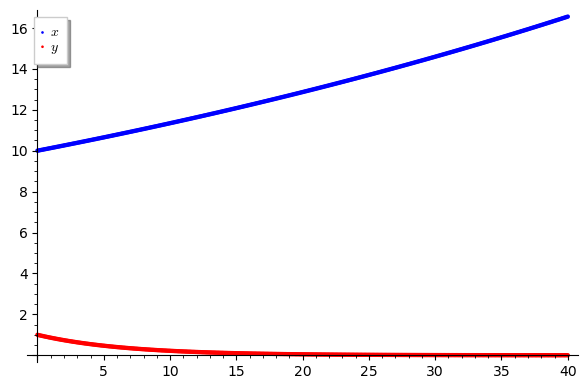
\includegraphics[scale=0.48]{figuras/LV_2.png}
        \label{fig:LV_2}
        \caption{$x_0 = 10$ e $y_0 = 1$}
    \end{subfigure}
    \begin{subfigure}{0.4\textwidth}
        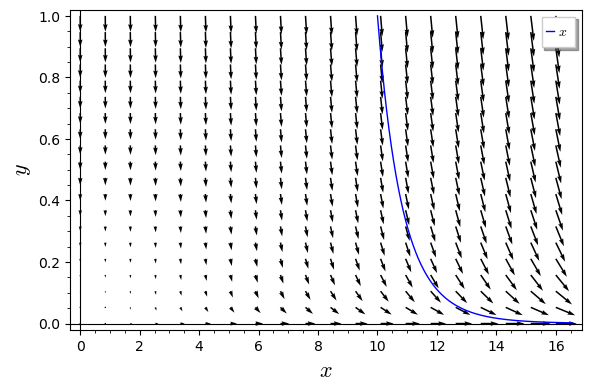
\includegraphics[scale=0.48]{figuras/LV_5.png}
        \label{fig:LV_5}
        \caption{Plano de fase}
    \end{subfigure}
\end{figure}

\begin{figure}[H]
    \centering
    \begin{subfigure}{0.4\textwidth}
        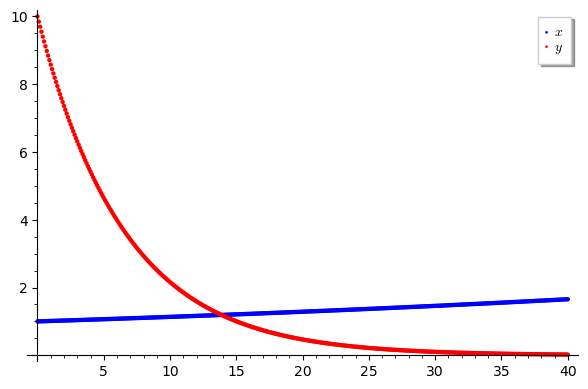
\includegraphics[scale=0.48]{figuras/LV_3.png}
        \label{fig:LV_3}
        \caption{$x_0 = 1$ e $y_0 = 10$}
    \end{subfigure}
    \begin{subfigure}{0.4\textwidth}
        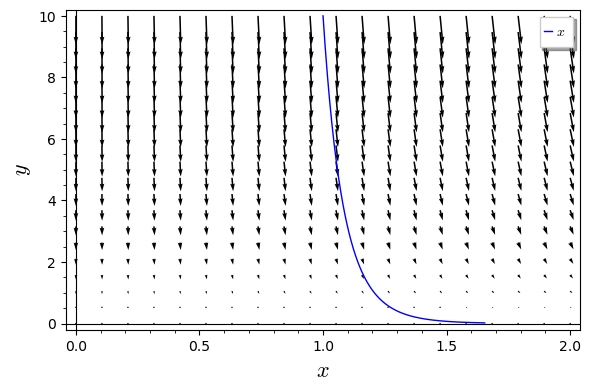
\includegraphics[scale=0.48]{figuras/LV_6.png}
        \label{fig:LV_6}
        \caption{Plano de fase}
    \end{subfigure}
\end{figure}

Quando variamos os parâmetros para $a = 0.0126, b = 0.01, c = 0.02, d = 0.0001$, vamos obter os seguintes gráficos.

\begin{figure}[H]
    \centering
    \begin{subfigure}{0.4\textwidth}
        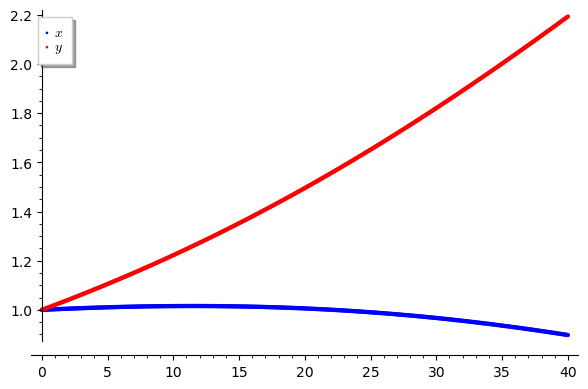
\includegraphics[scale=0.48]{figuras/LV_7.png}
        \label{fig:LV_7}
        \caption{$x_0 = y_0 = 1$}
    \end{subfigure}
    \begin{subfigure}{0.4\textwidth}
        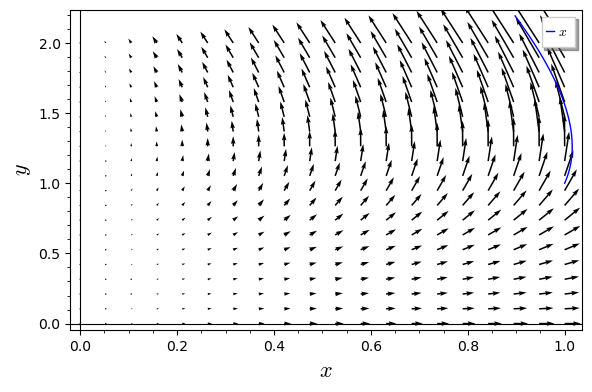
\includegraphics[scale=0.48]{figuras/LV_8.png}
        \label{fig:LV_8}
        \caption{Plano de fase}
    \end{subfigure}
\end{figure}

\begin{figure}[H]
    \centering
    \begin{subfigure}{0.4\textwidth}
        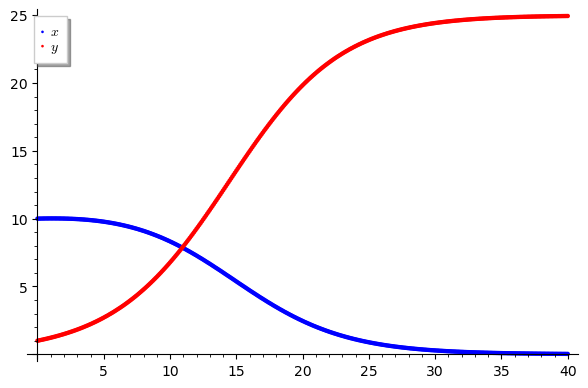
\includegraphics[scale=0.48]{figuras/LV_9.png}
        \label{fig:LV_9}
        \caption{$x_0 = 10$ e $y_0 = 1$}
    \end{subfigure}
    \begin{subfigure}{0.4\textwidth}
        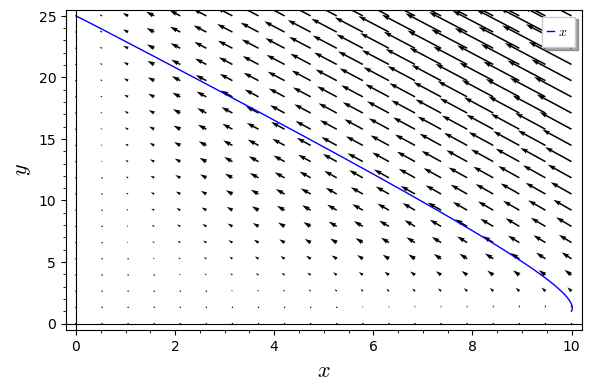
\includegraphics[scale=0.48]{figuras/LV_10.png}
        \label{fig:LV_10}
        \caption{Plano de fase}
    \end{subfigure}
\end{figure}

\begin{figure}[H]
    \centering
    \begin{subfigure}{0.4\textwidth}
        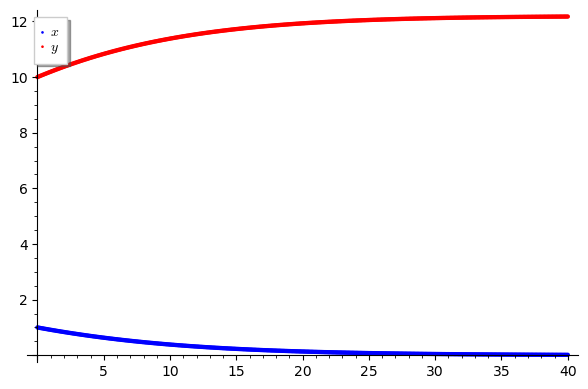
\includegraphics[scale=0.48]{figuras/LV_11.png}
        \label{fig:LV_11}
        \caption{$x_0 = 1$ e $y_0 = 10$}
    \end{subfigure}
    \begin{subfigure}{0.4\textwidth}
        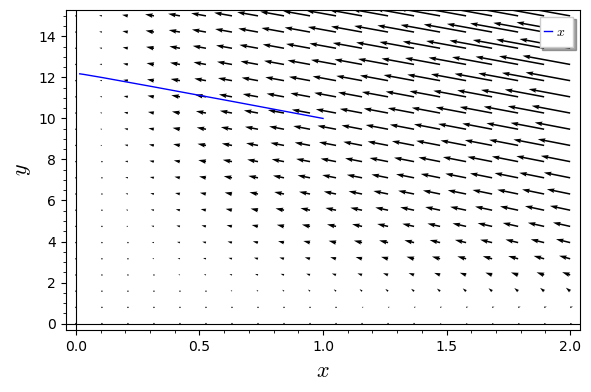
\includegraphics[scale=0.48]{figuras/LV_12.png}
        \label{fig:LV_12}
        \caption{Plano de fase}
    \end{subfigure}
\end{figure}

%%%%%%%%%%%%%%%%%%%%%%%%%%%%%%%%%%%%%%%%%%%%%%%%%%%%%%%%%%%
%%%%%%%%%%%%%%%%%%%%%%%%%%%%%%%%%%%%%%%%%%%%%%%%%%%%%%%%%%%
%%%%%%%%%%%%%%%%%%%% Modelo H-T %%%%%%%%%%%%%%%%%%%%%%%%%%%
%%%%%%%%%%%%%%%%%%%%%%%%%%%%%%%%%%%%%%%%%%%%%%%%%%%%%%%%%%%
%%%%%%%%%%%%%%%%%%%%%%%%%%%%%%%%%%%%%%%%%%%%%%%%%%%%%%%%%%%

\subsubsection{Modelo de Holling-Tanner}

Para esse modelo, os parâmetros foram calculados por M. S. Peixoto, L. C. Barros, e R. C. Bassanezi, no artigo produzido por eles \cite{mp_lb_rb_2005} (2005): $A = 10, K = 200, r = 2, m = 30.625, s = 0.3, c = 22.142857$. Nesse caso, temos os equilíbrios $P_1 = \left(0,0 \right), P_2 = \left( 200, 0 \right), P_3 = \left( -10, 0 \right), P_4 \approx \left( -25,806; -1,165 \right)$ e $P_5 \approx \left( 77,5; 3,5 \right)$, onde $P_2$ e $P_4$ são pontos de sela e $P_5$, uma espiral instável. A seguir, tem-se a simulação para diferentes condições iniciais e seus respectivos planos de fase.

\begin{figure}[H]
    \centering
    \begin{subfigure}{0.4\textwidth}
        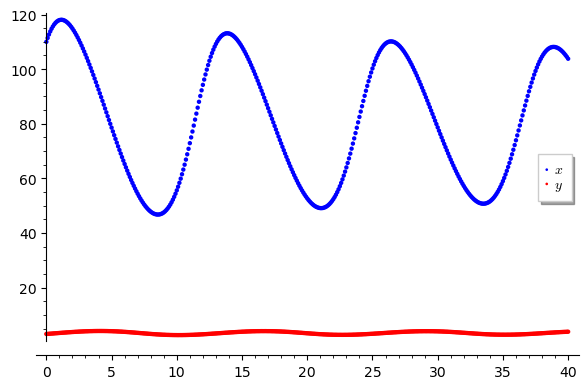
\includegraphics[scale=0.48]{figuras/HT_1.png}
        \label{fig:HT_1}
        \caption{$x_0 = 110$ e $y_0 = 3$}
    \end{subfigure}
    \begin{subfigure}{0.4\textwidth}
        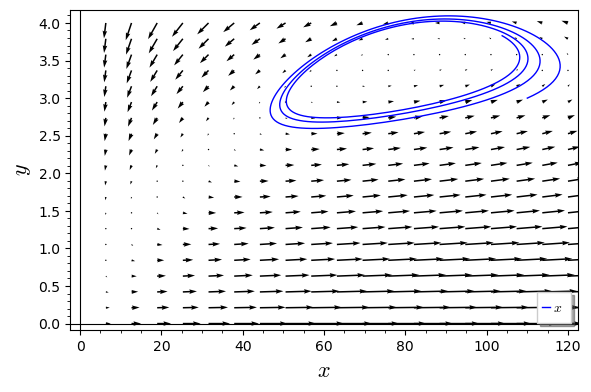
\includegraphics[scale=0.48]{figuras/HT_2.png}
        \label{fig:HT_2}
        \caption{Plano de fase}
    \end{subfigure}
\end{figure}

\begin{figure}[H]
    \centering
    \begin{subfigure}{0.4\textwidth}
        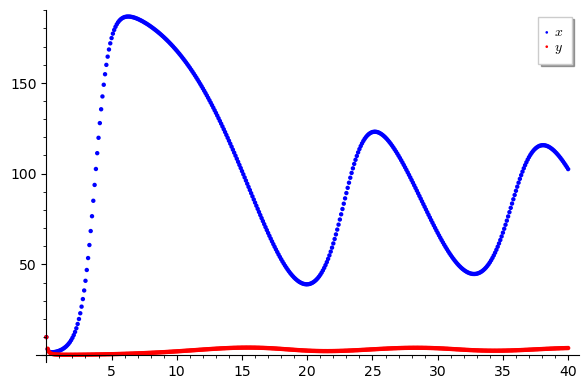
\includegraphics[scale=0.48]{figuras/HT_3.png}
        \label{fig:HT_3}
        \caption{$x_0 = y_0 = 10$}
    \end{subfigure}
    \begin{subfigure}{0.4\textwidth}
        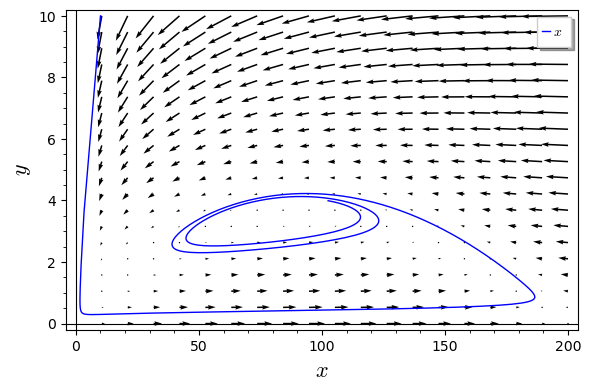
\includegraphics[scale=0.48]{figuras/HT_4.png}
        \label{fig:HT_4}
        \caption{Plano de fase}
    \end{subfigure}
\end{figure}

\begin{figure}[H]
    \centering
    \begin{subfigure}{0.4\textwidth}
        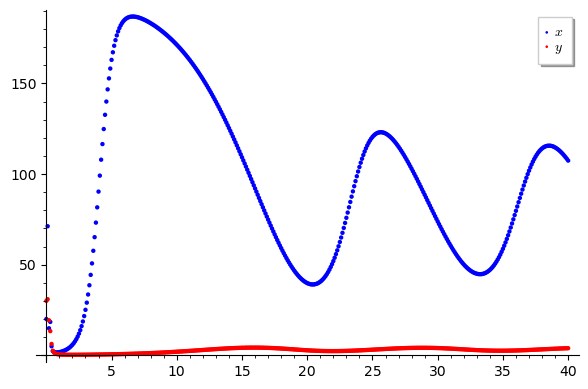
\includegraphics[scale=0.48]{figuras/HT_5.png}
        \label{fig:HT_5}
        \caption{$x_0 = 20$ e $y_0 = 30$}
    \end{subfigure}
    \begin{subfigure}{0.4\textwidth}
        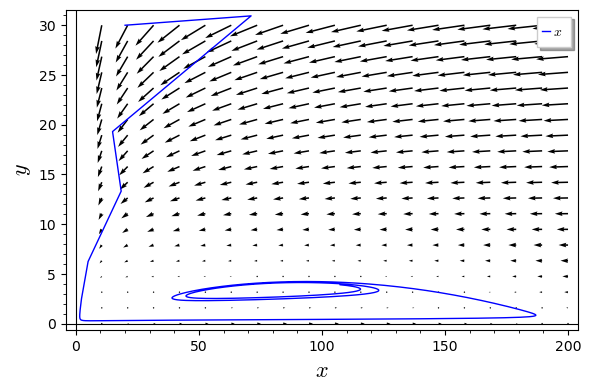
\includegraphics[scale=0.48]{figuras/HT_6.png}
        \label{fig:HT_6}
        \caption{Plano de fase}
    \end{subfigure}
\end{figure}

Quando aumentamos $s$ para $0.8$ e diminuímos $r$ para $1$, temos as seguintes figuras:

\begin{figure}[H]
    \centering
    \begin{subfigure}{0.4\textwidth}
        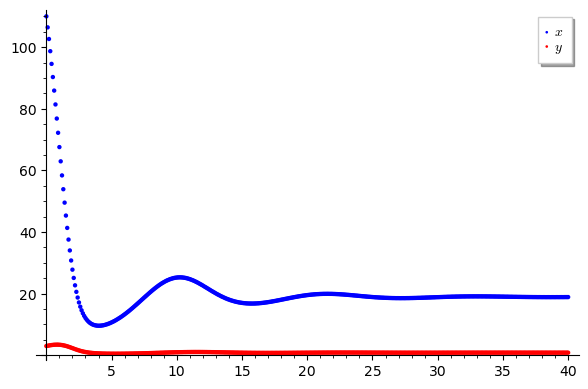
\includegraphics[scale=0.48]{figuras/HT_7.png}
        \label{fig:HT_7}
        \caption{$x_0 = 110$ e $y_0 = 3$}
    \end{subfigure}
    \begin{subfigure}{0.4\textwidth}
        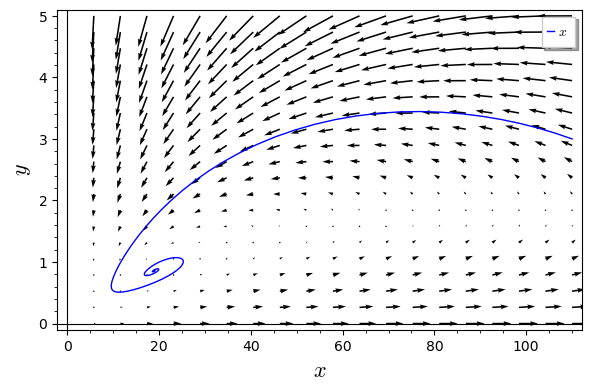
\includegraphics[scale=0.48]{figuras/HT_8.png}
        \label{fig:HT_8}
        \caption{Plano de fase}
    \end{subfigure}
\end{figure}

\begin{figure}[H]
    \centering
    \begin{subfigure}{0.4\textwidth}
        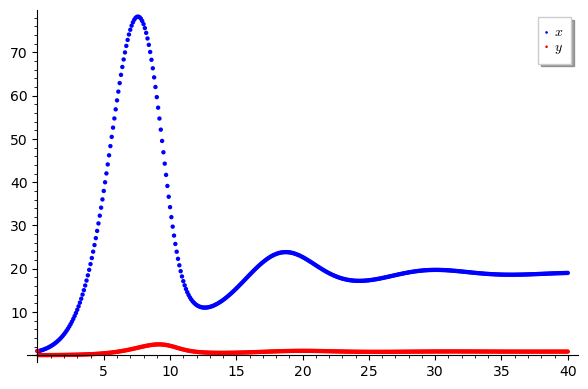
\includegraphics[scale=0.48]{figuras/HT_9.png}
        \label{fig:HT_9}
        \caption{$x_0 = y_0 = 1$}
    \end{subfigure}
    \begin{subfigure}{0.4\textwidth}
        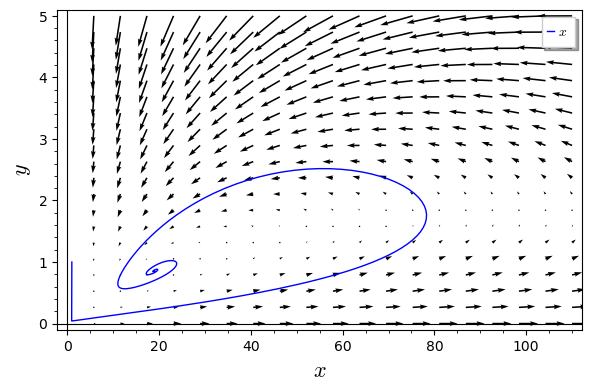
\includegraphics[scale=0.48]{figuras/HT_10.png}
        \label{fig:HT_10}
        \caption{Plano de fase}
    \end{subfigure}
\end{figure}

\begin{figure}[H]
    \centering
    \begin{subfigure}{0.4\textwidth}
        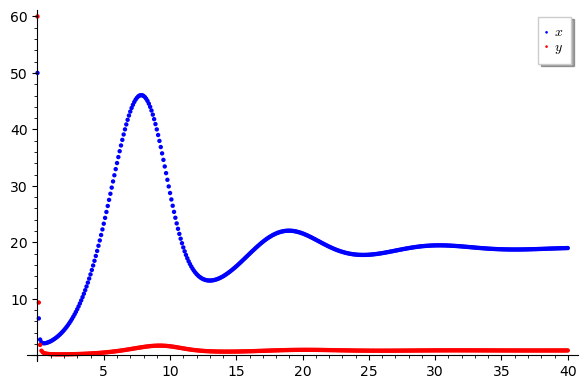
\includegraphics[scale=0.48]{figuras/HT_11.png}
        \label{fig:HT_11}
        \caption{$x_0 = 50$ e $y_0 = 60$}
    \end{subfigure}
    \begin{subfigure}{0.4\textwidth}
        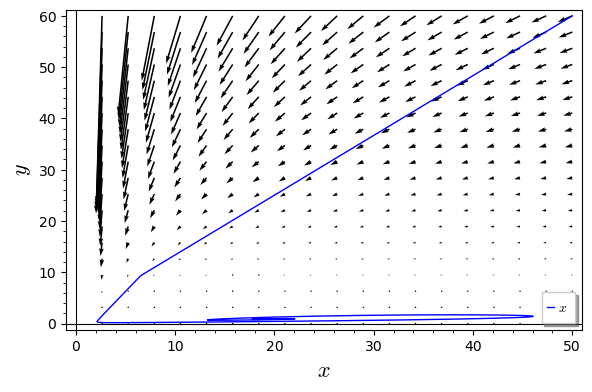
\includegraphics[scale=0.48]{figuras/HT_12.png}
        \label{fig:HT_12}
        \caption{Plano de fase}
    \end{subfigure}
\end{figure}

Por outro lado, aumentando também $m$ para $50$ e diminuindo $A$ para $5$, temos as seguintes figuras:

\begin{figure}[H]
    \centering
    \begin{subfigure}{0.4\textwidth}
        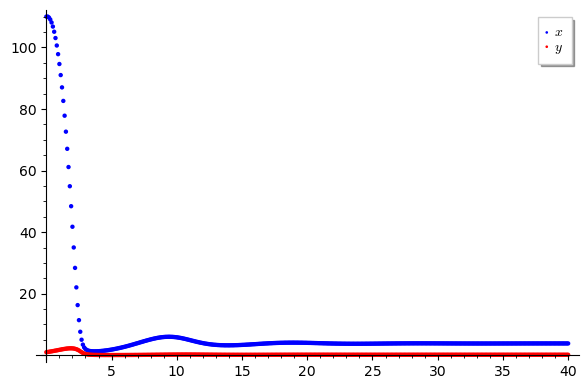
\includegraphics[scale=0.48]{figuras/HT_13.png}
        \label{fig:HT_13}
        \caption{$x_0 = 110$ e $y_0 = 1$}
    \end{subfigure}
    \begin{subfigure}{0.4\textwidth}
        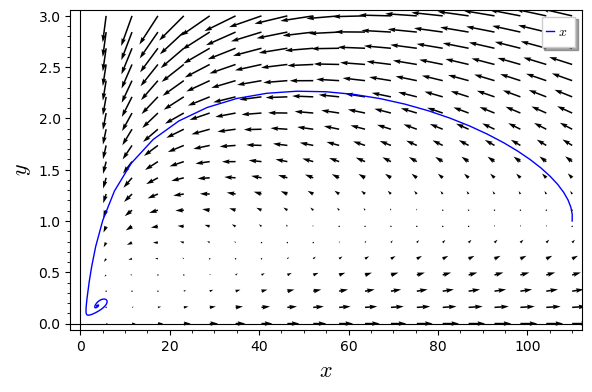
\includegraphics[scale=0.48]{figuras/HT_14.png}
        \label{fig:HT_14}
        \caption{Plano de fase}
    \end{subfigure}
\end{figure}

\begin{figure}[H]
    \centering
    \begin{subfigure}{0.4\textwidth}
        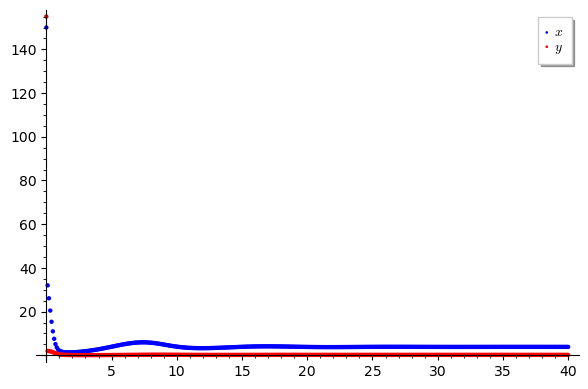
\includegraphics[scale=0.48]{figuras/HT_15.png}
        \label{fig:HT_15}
        \caption{$x_0 = 150$ e $y_0 = 155$}
    \end{subfigure}
    \begin{subfigure}{0.4\textwidth}
        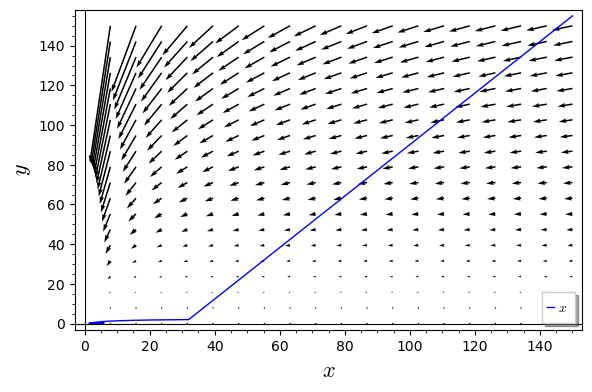
\includegraphics[scale=0.48]{figuras/HT_16.png}
        \label{fig:HT_16}
        \caption{Plano de fase}
    \end{subfigure}
\end{figure}

\begin{figure}[H]
    \centering
    \begin{subfigure}{0.4\textwidth}
        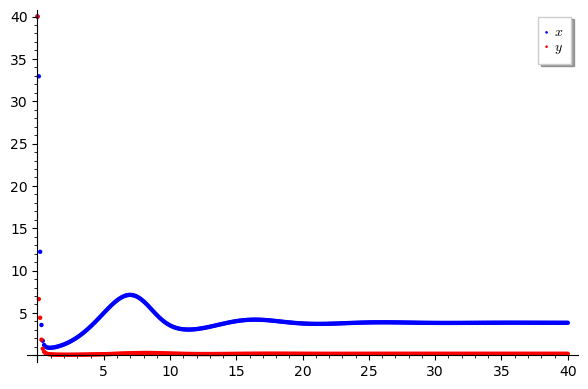
\includegraphics[scale=0.48]{figuras/HT_17.png}
        \label{fig:HT_17}
        \caption{$x_0 = y_0 = 40$}
    \end{subfigure}
    \begin{subfigure}{0.4\textwidth}
        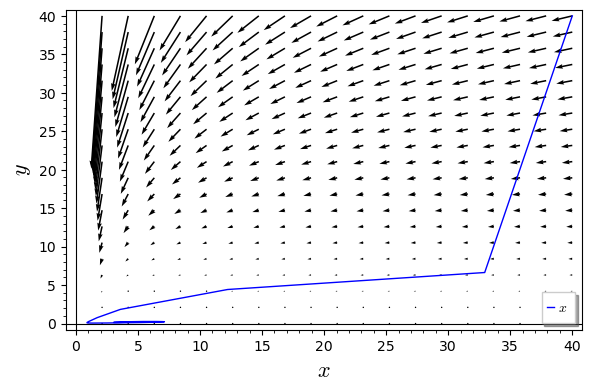
\includegraphics[scale=0.48]{figuras/HT_18.png}
        \label{fig:HT_18}
        \caption{Plano de fase}
    \end{subfigure}
\end{figure}

%%%%%%%%%%%%%%%%%%%%%%%%%%%%%%%%%%%%%%%%%%%%%%%%%%%%%%%%%%%
%%%%%%%%%%%%%%%%%%%%%%%%%%%%%%%%%%%%%%%%%%%%%%%%%%%%%%%%%%%
%%%%%%%%%%%%%%%%%%%% Modelo R-M %%%%%%%%%%%%%%%%%%%%%%%%%%%
%%%%%%%%%%%%%%%%%%%%%%%%%%%%%%%%%%%%%%%%%%%%%%%%%%%%%%%%%%%
%%%%%%%%%%%%%%%%%%%%%%%%%%%%%%%%%%%%%%%%%%%%%%%%%%%%%%%%%%%

\subsubsection{Modelo de Rosenzweig-MacArthur}

Nesse modelo, os parâmetros usados para o caso vespa-broca foram $A=5$, $K=100$, $r=1$, $m=15$, $s=0.45$ e $c=0.8$, testados nas populações iniciais $(x,y)=\{(1,1),(1,10),(10,1)\}$.

\begin{figure}[H]
    \centering
    \begin{subfigure}{0.4\textwidth}
        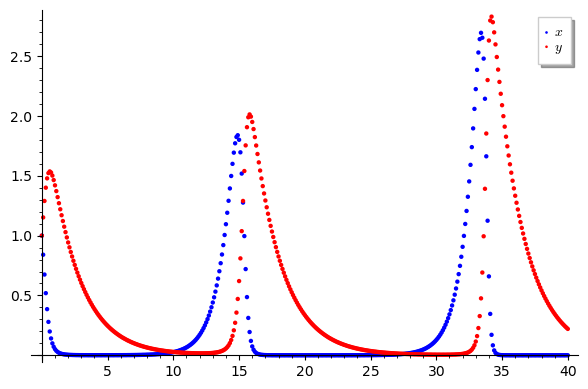
\includegraphics[scale=0.48]{figuras/RM-cana (1,1) plot.png}
        \label{fig:RM-cana_1}
        \caption{$x_0 = y_0 = 1$}
    \end{subfigure}
    \begin{subfigure}{0.4\textwidth}
        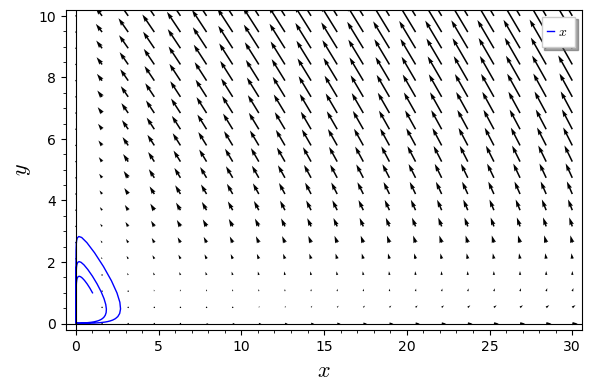
\includegraphics[scale=0.48]{figuras/RM-cana (1,1) plano.png}
        \label{fig:RM-cana_2}
        \caption{Plano de fase}
    \end{subfigure}
\end{figure}

\begin{figure}[H]
    \centering
    \begin{subfigure}{0.4\textwidth}
        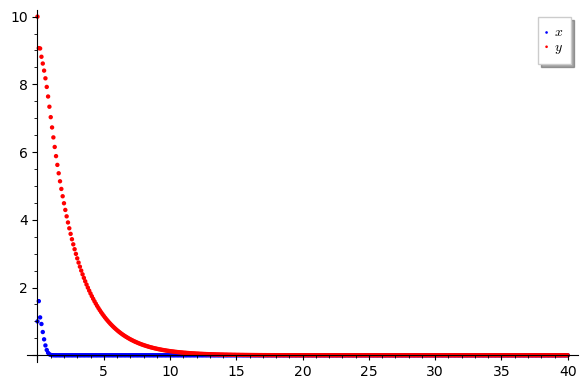
\includegraphics[scale=0.48]{figuras/RM-cana (1,10) plot.png}
        \label{fig:RM-cana_3}
        \caption{$x_0 = 1$ e $y_0 = 10$}
    \end{subfigure}
    \begin{subfigure}{0.4\textwidth}
        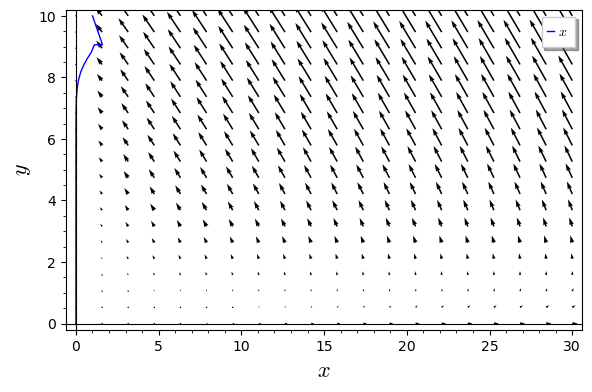
\includegraphics[scale=0.48]{figuras/RM-cana (1,10) plano.png}
        \label{fig:RM-cana_4}
        \caption{Plano de fase}
    \end{subfigure}
\end{figure}

\begin{figure}[H]
    \centering
    \begin{subfigure}{0.4\textwidth}
        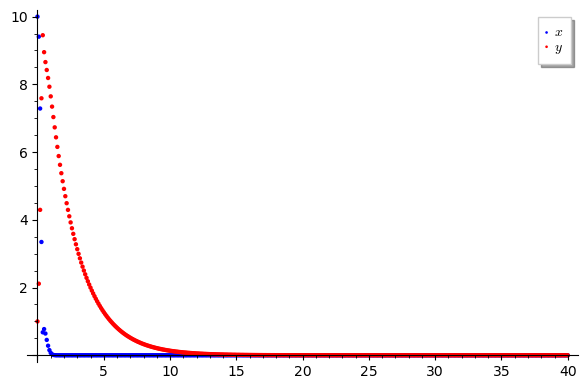
\includegraphics[scale=0.48]{figuras/RM-cana (10,1) plot.png}
        \label{fig:RM-cana_5}
        \caption{$x_0 = 10$ e $y_0 = 1$}
    \end{subfigure}
    \begin{subfigure}{0.4\textwidth}
        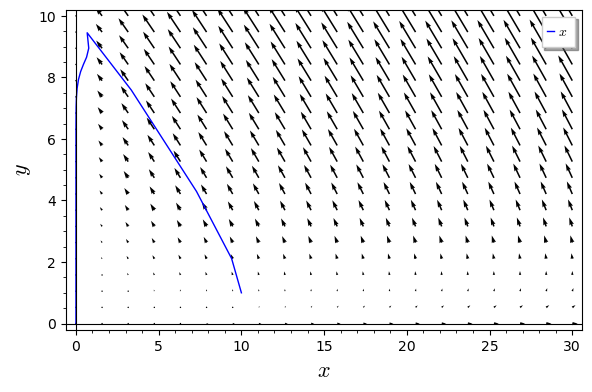
\includegraphics[scale=0.48]{figuras/RM-cana (10,1) plano.png}
        \label{fig:RM-cana_6}
        \caption{Plano de fase}
    \end{subfigure}
\end{figure}

Já no sistema joaninha-pulgão, os parâmetros utilizados foram $A=10$, $K=200$, $r=2$, $m=30.625$, $s=0.5$ e $c=1$, testados nas mesmas populações iniciais do caso anterior, $(x,y)=\{(1,1),(1,10),(10,1)\}$.

\begin{figure}[H]
    \centering
    \begin{subfigure}{0.4\textwidth}
        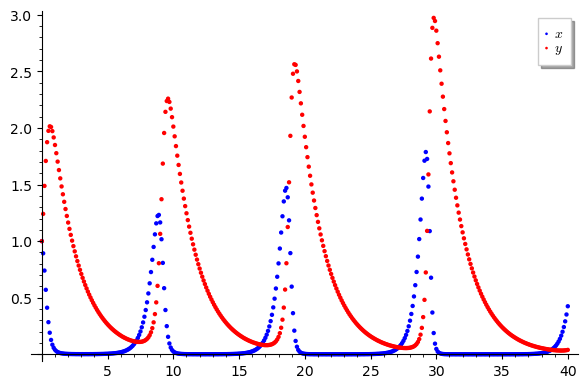
\includegraphics[scale=0.48]{figuras/RM-citros (1,1) plot.png}
        \label{fig:RM-citros_1}
        \caption{$x_0 = y_0 = 1$}
    \end{subfigure}
    \begin{subfigure}{0.4\textwidth}
        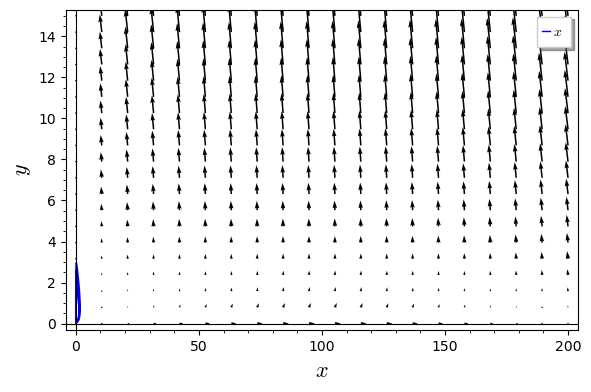
\includegraphics[scale=0.48]{figuras/RM-citros (1,1) plano.png}
        \label{fig:RM-citros_2}
        \caption{Plano de fase}
    \end{subfigure}
\end{figure}

\begin{figure}[H]
    \centering
    \begin{subfigure}{0.4\textwidth}
        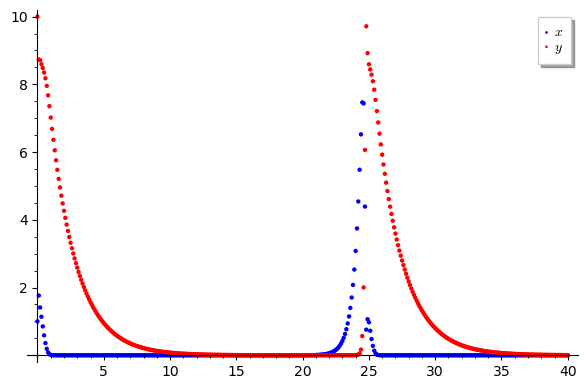
\includegraphics[scale=0.48]{figuras/RM-citros (1,10) plot.png}
        \label{fig:RM-citros_3}
        \caption{$x_0 = 1$ e $y_0 = 10$}
    \end{subfigure}
    \begin{subfigure}{0.4\textwidth}
        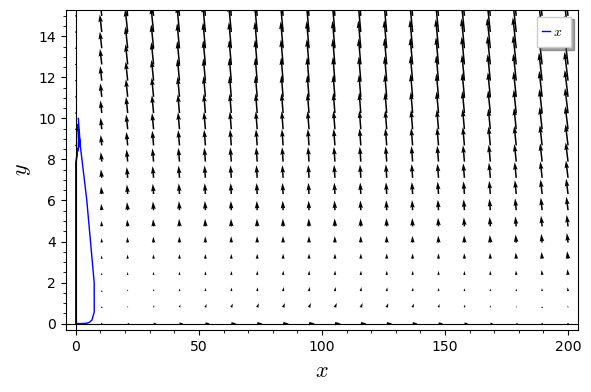
\includegraphics[scale=0.48]{figuras/RM-citros (1,10) plano.png}
        \label{fig:RM-citros_4}
        \caption{Plano de fase}
    \end{subfigure}
\end{figure}

\begin{figure}[H]
    \centering
    \begin{subfigure}{0.4\textwidth}
        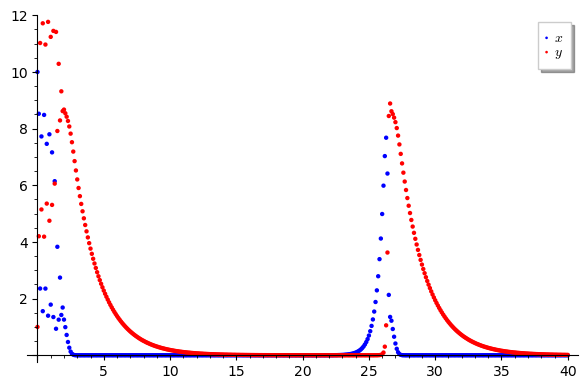
\includegraphics[scale=0.48]{figuras/RM-citros (10,1) plot.png}
        \label{fig:RM-citros_5}
        \caption{$x_0 = 10$ e $y_0 = 1$}
    \end{subfigure}
    \begin{subfigure}{0.4\textwidth}
        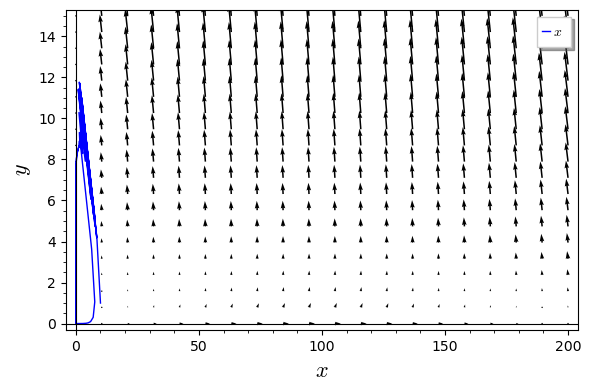
\includegraphics[scale=0.48]{figuras/RM-citros (10,1) plano.png}
        \label{fig:RM-citros_6}
        \caption{Plano de fase}
    \end{subfigure}
\end{figure}

A maneira como foi feita a estimação desses parâmetros será discutida na próxima seção.

% \newpage

% \section{Discussão}
% \newpage

% \section{Conclusão}

Analisamos três modelos com o intuito de modelar a dinâmica predador-presa nas populações de brocas e vespas e de pulgões e joaninhas. Com o modelo de Lotka-Volterra, fizemos uma representação simplificada para as primeiras populações, onde o modelo pressupõe crescimento indefinido das espécies. Em seguida, exploramos o modelo de Holling-Tanner com as populações de pulgões e joaninhas, onde pudemos contemplar uma maior representação da realidade, com o crescimento das populações limitado e dependente das interações entre elas. Por fim, tentamos modelar ambas as dinâmicas populacionais com o modelo de Rosenzweig-MacArthur, semelhante ao modelo anterior, mas que considera outras características dos predadores. Nesse modelo, percebemos um comportamento bem cíclico, onde a população de presas crescia à medida que a população de predadores diminuía.

A abordagem aqui presente se mostra de suma importância para estudar a dinâmica das populações e buscar maneiras efetivas de estabelecer um controle biológico das presas. No entanto, o grande fator limitante é a ausência de dados para a estimação dos parâmetros utilizados. Sobretudo no último modelo, devido a falta de muitos deles, tivemos que definir algumas condições de regularidade para a realização da modelagem. Ademais, esbarramos na limitação de estabilidade numérica, onde precisamos determinar intervalos de estimação dos parâmetros condizentes com a realidade e que eram estáveis numericamente.

% \newpage

\nocite{*}
\bibliographystyle{IEEEtran}
\bibliography{bibliografia/referencias}

\end{document}
